\chapter{Poetry}

\epigraph{"Carpe diem. Seize the day, boys. Make your lives extraordinary."}{---John Keating, Dead Poets Society (1989)}

\newcommand{\garden}{
I used to love my garden \\
But now my love is dead \\
For I found a bachelor's button \\
In black-eyed Susan's bed.
}
Typographical standards require poetry to be `'centered on the longest line, unless such line is disproportionately long, in which case optical centring''. \textit{The oxford Dictionary for Writers and Editors}, which presents the house style of
the Oxford University Press). 


\section{Using the verse package}



\begin{lstlisting}[language={[common]TeX},% 
                           alsolanguage={[LaTeX]TeX},% 
                           alsolanguage={[primitive]TeX},%
                           alsolanguage={extras}]
\renewcommand{\poemtoc}{subsection}
\poemtitle{A Limerick}
\settowidth{\versewidth}{There was an old party of Lyme}
\begin{verse}[\versewidth]
    There was an old party of Lyme \\
    Who married three wives at one time. \\
    \vin When asked: `Why the third?' \\
    \vin He replied: `One's absurd, \\
    And bigamy, sir, is a crime.'
\end{verse}
\end{lstlisting}


which gets typeset as below. The default \doccmd{poemtoc}  is redefined to subsection so
the title is entered into the ToC as an unnumbered subsection.

\newlength{\aaaa}
\settowidth{\aaaa}{ZZZZ}

\renewcommand{\poemtoc}{subsection}
\poemtitle{A Limerick}
\settowidth{\versewidth}{There was an old party of Lyme}
\begin{verse}[\versewidth]
    There was an old party of Lyme \\
     Who married three wives at one time. \\
    \vin When asked: `Why the third?' \\
    \ZZZZ He replied: `One's absurd, \\
And bigamy, sir, is a crime.'
\end{verse}

Next is the Garden verse within the altverse environment. It is titled and
centered.

\settowidth{\versewidth}{But now my love is dead}
\poemtitle{Love's lost}
\begin{verse}[\versewidth]
\begin{altverse}
\garden
\end{altverse}
\end{verse}


which produces:

\settowidth{\versewidth}{But now my love is dead}
\poemtitle{Love's lost}
\begin{verse}[\versewidth]
    \begin{altverse}
    \garden
\end{altverse}
\end{verse}


It is left up to you how you might want to add information about the author
of a poem. Here is one example of a macro for this:

\begin{lstlisting}[language={[common]TeX},% 
                           alsolanguage={[LaTeX]TeX},% 
                           alsolanguage={[primitive]TeX},%
                           alsolanguage={extras}]
\newcommand{\attrib}[1]{%
\nopagebreak{\raggedleft\footnotesize #1\par}}
\end{lstlisting}

\newcommand{\attrib}[1]{%
\nopagebreak{\raggedleft\footnotesize #1\par}}
This can be used as in the next bit of doggeral.

\poemtitle{Fleas}
\settowidth{\versewidth}{What a funny thing is a flea}
\begin{verse}[\versewidth]
What a funny thing is a flea. \\
You can't tell a he from a she. \\
 But he can. And she can. \\
 Whoopee!
\end{verse}
\attrib{Anonymous}


Here is an example of line wrapping.
\poemtitle{In the beginning}
\settowidth{\versewidth}{And objects at rest tended to remain at rest}
\begin{verse}[\versewidth]
Then God created Newton, \\*
And objects at rest tended to remain at rest, \\*
And objects in motion tended to remain in motion, \\*
And energy was conserved
and momentum was conserved
and matter was conserved \\*
And God saw that it was conservative.
\end{verse}
\attrib{Possibly from \textit{Analog}, circa 1950}



Here is one with a forced line break and a slightly different title style.

\begin{lstlisting}[language={[common]TeX},% 
                           alsolanguage={[LaTeX]TeX},% 
                           alsolanguage={[primitive]TeX},%
                           alsolanguage={extras}]
\renewcommand{\poemtitlefont}{\normalfont\large\itshape\centering}
\poemtitle{Mathematics}
\settowidth{\versewidth}{Than Tycho Brahe, or Erra Pater:}
\begin{verse}[\versewidth]
    In mathematics he was greater \\
    Than Tycho Brahe, or Erra Pater: \\
    For he, by geometric scale, \\
   Could take the size of pots of ale;\\ \settowidth{\versewidth}{Resolve by}
   Resolve, by sines \\>[\versewidth] and tangents straight, \\
   If bread or butter wanted weight; \\
   And wisely tell what hour o' the day \\
   The clock does strike, by Algebra.
\end{verse}
\attrib{Samuel Butler (1612--1680)}
\end{lstlisting}

The typesetting now is slightly different but still not what is probably required in a poetry book

\begin{verse}[\versewidth]
    In mathematics he was greater \\
    Than Tycho Brahe, or Erra Pater: \\
    For he, by geometric scale, \\
   Could take the size of pots of ale;\\ \settowidth{\versewidth}{Resolve by}
   Resolve, by sines \\>[\versewidth] and tangents straight, \\
   If bread or butter wanted weight; \\
   And wisely tell what hour o' the day \\
   The clock does strike, by Algebra.
\end{verse}
\attrib{Samuel Butler (1612--1680)}
\bigskip


Another limerick, but this time taking advantage of the patverse environment
and numbering every third line.

\begin{lstlisting}[language={[common]TeX},% 
                           alsolanguage={[LaTeX]TeX},% 
                           alsolanguage={[primitive]TeX},%
                           alsolanguage={extras}]
\settowidth{\versewidth}{There was a young lady of Ryde}
\poemtitle{The Young Lady of Ryde}
\begin{verse}[\versewidth]
\poemlines{3}
\indentpattern{00110}
\begin{patverse}
There was a young lady of Ryde \\
Who ate some apples and died. \\
The apples fermented \\
Inside the lamented \\
And made cider inside her inside.
\end{patverse}
\poemlines{0}
\end{verse}
\end{lstlisting}


The  poem on the next page is a bit more involved. Here we use a bigskip between the verses of the poem. Also note
the use of the emdash, which is commonly found in poetry books. The command \doccmd{vin} is from the verse class
and it justs sets the second line in. The figure which is from the same publication was set with a marginfigure and the
vertical height was manually adjusted. Poetry typesetting is highly unlikely to be done automatically. Each poem is
special and would normally be typset to suit.

\begin{lstlisting}[language={[common]TeX},% 
                           alsolanguage={[LaTeX]TeX},% 
                           alsolanguage={[primitive]TeX},%
                           alsolanguage={extras}]
\begin{verse}[\versewidth]
   See the beetle that crawls in your way,\\
  \vin And runs to escape from your feet;\\
   His house is a hole in the clay,\\
   \vin And the bright morning dew is his meat.\\
\bigskip
   But if you more closely behold\\
   \vin This insect you think is so mean,\\
   You will find him all spangled with gold,\\
  \vin And shining with crimson and green.\\
\end{Verse}
\end{lstlisting}

\clearpage
\poemtitle{THE BEETLE}
\marginpar{%
\hspace*{-30pt}\hbox to 0pt{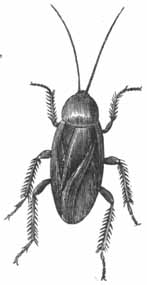
\includegraphics[width=100pt]{./images/beetle.jpg}}
  \label{fig:beetle}
}

\begin{verse}[\versewidth]
See the beetle that crawls in your way,\\
\vin And runs to escape from your feet;\\
His house is a hole in the clay,\\
\vin And the bright morning dew is his meat.\\
\bigskip
But if you more closely behold\\
\vin This insect you think is so mean,\\
You will find him all spangled with gold,\\
\vin And shining with crimson and green.\\
\bigskip
Tho' the peacock's bright plumage we prize,\\
\vin As he spreads out his tail to the sun,\\
The beetle we should not despise,\\
\vin Nor over him carelessly run.\\
\bigskip
They both the same Maker declare---\\
\vin They both the same wisdom display,\\
The same beauties in common they share---\\
\vin Both are equally happy and gay.\\
\bigskip
And remember that while you would fear\\
\vin The beautiful peacock to kill,\\
You would tread on the poor beetle here,\\
\vin And think you were doing no ill.\\
\bigskip
But though 'tis so humble, be sure,\\
\vin As mangled and bleeding it lies,\\
A pain as severe 'twill endure,\\
\vin As if 'twere a giant that dies\sidenote{Anonymous, \textit{Illustrared London Book} 1851}.\\
\end{verse}

\clearpage
\marginpar{%
 \includegraphics[width=80pt]{./images/byron.jpg}
  \label{fig:beetle}
}
\poemtitle{ON JORDAN'S BANKS}
\begin{verse}[\versewidth]
On Jordan's banks the Arab camels stray,\\
On Sion's hill the False One's votaries pray---\\
The Baal-adorer bows on Sinai's steep;\\
Yet there---even there---O God! thy thunders sleep:\\
\bigskip
There, where thy finger scorch'd the tablet stone;\\
There, where thy shadow to thy people shone---\\
Thy glory shrouded in its garb of fire\\
(Thyself none living see and not expire).\\
\bigskip
Oh! in the lightning let thy glance appear---\\
Sweep from his shiver'd hand the oppressor's spear!\\
How long by tyrants shall thy land be trod?\\
How long thy temple worshipless, O God!\\
\end{verse}



\begin{comment}
 \clearpage
 \poemtitle{Mouse's Tale}
 \settowidth{\versewidth}{a mouse that morning}
 \indentpattern{0135554322112346898779775545653222345544456688778899}
 \begin{verse}[\versewidth]
 \setlength{\vgap}{1em}
 \begin{patverse}
 \large Fury said to \\
   a mouse, That \\
   he met \\
   in the \\
   house, \\
 \normalsize `Let us \\
   both go \\
   to law: \\
   \emph{I} will \\
   prosecute \\
   \textit{you.} --- \\ 
   Come, I'll \\
 \small take no \\
   denial; \\
   We must \\
   have a \\
   trial: \\
   For \\
 \footnotesize really \\
   this \\
   morning \\
   I've \\
   nothing \\
   to do.' \\
   Said the \\
   mouse to \\
 \scriptsize the cur, \\
   Such a \\
   trial, \\
   dear sir, \\
   With no \\
   jury or \\
   judge, \\
   would be \\
   wasting \\
   our breath.' \\
 \tiny  `I'll be \\
   judge, \\
   I'll be \\
   jury.' \\
   Said \\
   cunning \\
   old Fury; \\
   `I'll try \\
   the whole \\
   cause \\
   and \\
   condemn \\
   you \\
   to \\
   death.'  \par
 \end{patverse}
 \end{verse}
 \attrib{Lewis Carrol, \textit{Alice's Adventures in Wonderland}, 1865}
 
\clearpage
\end{comment}


 Using the |alltt| environment you can put in the spacing via ordinary
 spaces. That is, this

\begin{lstlisting}[language={[common]TeX},% 
                           alsolanguage={[LaTeX]TeX},% 
                           alsolanguage={[primitive]TeX},%
                           alsolanguage={extras}]
 \begin{alltt}\normalfont
 There was an old party of Lyme
 Who married three wives at one time.
       When asked: `Why the third?' 
       He replied: `One's absurd, 
 And bigamy, sir, is a crime.'
 \end{alltt}
 \end{lstlisting}

 is typeset as

 \begin{alltt}
 \normalfont
 There was an old party of Lyme
 Who married three wives at one time.
       When asked: `Why the third?' 
       He replied: `One's absurd, 
 And bigamy, sir, is a crime.'
 \end{alltt}


\begin{codeexample}[]
\begin{tikzpicture}[scale=0.5]
\def \n {5}
\def \radius {3cm}
\def \margin {12} 

\foreach \s[count=\xi from 0] in {1,...,\n}
{
  \node[draw, circle] at ({360/\n * (\s - 1)}:\radius) {$\xi$};
  \draw[->, >=latex] ({360/\n * (\s - 1)+\margin}:\radius) 
    arc ({360/\n * (\s - 1)+\margin}:{360/\n * (\s)-\margin}:\radius);
}
\end{tikzpicture}
\end{codeexample}







